\documentclass[12pt,fleqn,unicode]{article}
\usepackage{Diplo}
\usepackage{tikz}
\usetikzlibrary{shapes,arrows,shadows}
\usepackage{subcaption}
\usepackage{subfig}

% \usepackage{graphicx}
%\usepackage{caption}
%\usepackage{subcaption}
%\usepackage[cp1251]{inputenc}
%\usepackage{amssymb,amsmath}
%\usepackage[russian]{babel}
%\usepackage{array}
%\usepackage[ruled,section]{algorithm}
%\usepackage[noend]{algorithmic}
%\usepackage[all]{xy}
%\usepackage{graphicx}
%\usepackage{indentfirst}
% \usepackage{bigstrut}
% \usepackage{float}
% \DeclareMathOperator*{\argmax}{arg\,max}

%\clubpenalty=10000
%\widowpenalty=10000
%% для больших плавающих иллюстраций
%\renewcommand\topfraction{1.0}
%\renewcommand\textfraction{0.0}
%\renewcommand\floatpagefraction{0.01} % float-страниц быть вообще не должно - это чтобы их лучше видеть ;)
% Воронцов
% \newcommand\brop[1]{#1\discretionary{}{\hbox{$\mathsurround=0pt #1$}}{}}
\newcommand{\tsum}{\mathop{\textstyle\sum}\limits}
\renewcommand{\geq}{\geqslant}
\renewcommand{\leq}{\leqslant}
\newcommand{\scal}[2]{\left\langle #1,#2 \right\rangle}
\def\XYtext(#1,#2)#3{\rlap{\kern#1\lower-#2\hbox{#3}}}

\newcommand{\executeiffilenewer}[3]{%
 \ifnum\pdfstrcmp{\pdffilemoddate{#1}}%
 {\pdffilemoddate{#2}}>0%
 {\immediate\write18{#3}}\fi%
}
\newcommand{\includesvg}[1]{%
 \executeiffilenewer{#1.svg}{#1.pdf}%
 {inkscape -z -D --file=#1.svg %
 --export-pdf=#1.pdf --export-latex}%
 \input{#1.pdf_tex}%
}
\usepackage{pb-diagram}
\usepackage{bm}

\graphicspath{ {./fig/} }

%%%%%%%%%%%%%%%%%%%%%%%%%%%%%%%%%%%%%%%%%%%%%%%%%%%%%%%%%%%%%%%%%%%%%%%%%%%%%%%
% Оформление алгоритмов в пакетах algorithm, algorithmic
%%%%%%%%%%%%%%%%%%%%%%%%%%%%%%%%%%%%%%%%%%%%%%%%%%%%%%%%%%%%%%%%%%%%%%%%%%%%%%%
% % переопределения (русификация) управляющих конструкций:
% \newcommand{\algKeyword}[1]{{\bf #1}}
\floatname{algorithm}{Алгоритм}
\renewcommand{\algorithmicrequire}{\rule{0pt}{2.5ex}{{\bf Вход:}}}
\renewcommand{\algorithmicensure}{{\bf Выход:}}
\renewcommand{\algorithmicend}{{\bf конец}}
\renewcommand{\algorithmicif}{{\bf если}}
\renewcommand{\algorithmicthen}{{\bf то}}
\renewcommand{\algorithmicelse}{{\bf иначе}}
\renewcommand{\algorithmicelsif}{\algorithmicelse\ \algorithmicif}
\renewcommand{\algorithmicendif}{\algorithmicend\ \algorithmicif}
\renewcommand{\algorithmicfor}{{\bf для}}
\renewcommand{\algorithmicforall}{{\bf для всех}}
\renewcommand{\algorithmicdo}{}
\renewcommand{\algorithmicendfor}{\algorithmicend\ \algorithmicfor}
\renewcommand{\algorithmicwhile}{{\bf пока}}
\renewcommand{\algorithmicendwhile}{\algorithmicend\ \algorithmicwhile}
\renewcommand{\algorithmicloop}{{\bf цикл}}
\renewcommand{\algorithmicendloop}{\algorithmicend\ \algorithmicloop}
\renewcommand{\algorithmicrepeat}{{\bf повторять}}
\renewcommand{\algorithmicuntil}{{\bf пока}}
%\renewcommand{\algorithmiccomment}[1]{{\footnotesize // #1}}
\renewcommand{\algorithmiccomment}[1]{{\quad\sl // #1}}

\newcommand{\bz}{\mathbf{z}}
\newcommand{\bx}{\mathbf{x}}
\newcommand{\by}{\mathbf{y}}
\newcommand{\bw}{\mathbf{w}}
\newcommand{\bY}{\mathbf{Y}}
\newcommand{\bX}{\mathbf{X}}
\newcommand{\ba}{\mathbf{a}}
\newcommand{\bu}{\mathbf{u}}
\newcommand{\bt}{\mathbf{t}}
\newcommand{\bp}{\mathbf{p}}
\newcommand{\bq}{\mathbf{q}}
\newcommand{\br}{\mathbf{r}}
\newcommand{\bg}{\mathbf{g}}
\newcommand{\bh}{\mathbf{h}}
\newcommand{\bb}{\mathbf{b}}
\newcommand{\bv}{\mathbf{v}}
\newcommand{\be}{\mathbf{e}}
\newcommand{\bc}{\mathbf{c}}
\newcommand{\bs}{\mathbf{s}}
\newcommand{\bP}{\mathbf{P}}
\newcommand{\bT}{\mathbf{T}}
\newcommand{\bQ}{\mathbf{Q}}
\newcommand{\bE}{\mathbf{E}}
\newcommand{\bF}{\mathbf{F}}
\newcommand{\bU}{\mathbf{U}}
\newcommand{\bI}{\mathbf{I}}
\newcommand{\bB}{\mathbf{B}}
\newcommand{\bW}{\mathbf{W}}
\newcommand{\bD}{\mathbf{D}}
\newcommand{\bH}{\mathbf{H}}
\newcommand{\bG}{\mathbf{G}}
\newcommand{\bZ}{\mathbf{Z}}
\newcommand{\bJ}{\mathbf{J}}
\newcommand{\bM}{\mathbf{M}}
\newcommand{\btheta}{\boldsymbol{\theta}}
\newcommand{\bmu}{\boldsymbol{\mu}}
\newcommand{\blambda}{\boldsymbol{\lambda}}
\newcommand{\bPsi}{\boldsymbol{\Psi}}
\newcommand{\bchi}{\boldsymbol{\chi}}
\newcommand{\bsigma}{\boldsymbol{\sigma}}
\newcommand{\bTheta}{\boldsymbol{\Theta}}
\newcommand{\bphi}{\boldsymbol{\phi}}
\newcommand{\bdelta}{\boldsymbol{\delta}}

\newcommand{\T}{^{\text{\tiny\sffamily\upshape\mdseries T}}}



\begin{document}

{
\renewcommand{\baselinestretch}{1}
\thispagestyle{empty}
\begin{center}
    \sc
        Министерство образования и науки Российской Федерации\\
        Московский физико-технический институт
        {\rm(государственный университет)}\\
        Факультет управления и прикладной математики\\
        Кафедра <<Интеллектуальные системы>>\\
        при Вычислительном центре им. А. А. Дородницына РАН\\[35mm]
    \rm\large
        Владимирова Мария Руслановна\\[10mm]
    \bf\Large
    Снижение размерности пространства зависимой переменной\\[10mm]
    \rm\normalsize
        010900 — Прикладные математика и физика\\[10mm]
    \sc
        Выпускная квалификационная работа бакалавра\\[30mm]
\end{center}
\hfill\parbox{80mm}{
    \begin{flushleft}
    \bf
        Научный руководитель:\\
    \rm
        д.ф.-м.н. Стрижов Вадим Викторович\\[4.9cm]
    \end{flushleft}
}
\begin{center}
    Москва\\
    2017 г.
\end{center}
}

\newpage
\tableofcontents

%%%%%%%%%%%%%%%%%%%%%%%%%%%%%%%%%%%%%%%%%%%%%%%%%%%%%%%%%%%%%%%%%%%%%%%%%%%%%%
\newpage
\begin{abstract}
  Решается задача обнаружения способов зависимостей в прогнозируемой переменной. Используется набор гомогенных моделей, восстанавливающих прогноз по общему для всех переменных описанию объектов. Анализируется различие в пространстве параметров моделей. По результатам анализа выбирается оптимальная структура каждой модели. Проводится эксперимент на реальных данных объемов потребления электроэнергии для сравнения предложенных методов.  

  \bigskip
    \textbf{Ключевые слова}: \emph{прогнозирование временных рядов; мультиколлинеарность; матод частных наименьших квадратов; PLS; нелинейный PLS.}
\end{abstract}

%%%%%%%%%%%%%%%%%%%%%%%%%%%%%%%%%%%%%%%%%%%%%%%%%%%%%%%%%%%%%%%%%%%%%%%%%%%%%%
\newpage
\section{Введение}
%%%%%%%%%%%%%%%%%%%%%%%%%%%%%%%%%%%%%%%%%%%%%%%%%%%%%%%%%%%%%%%%%%%%%%%%%%%%%%
% В рассматривается рассматривается проблема проектирования Brain-Computer Interface (BCI). Мы решаем проблему выбора функций в моделях регрессии в приложении к декодированию движения на основе электрокардиограмм (ЭКГ). Задача состоит в том, чтобы предсказать траектории руки из временных рядов напряжения кортикальной активности. Описание функции каждой точки находится в пространственно-временной частотной области и включает в себя сами временные ряды напряжения и их спектральные характеристики. Выбор функции имеет решающее значение для адекватного решения проблемы регрессии, поскольку электрокортикальные данные являются высокомерными и измерения коррелируют как во временной, так и в пространственной областях.


% Система Brain-Computer Interface (BCI) улучшает умственные и физические возможности пользователя, обеспечивая прямую связь между мозгом и компьютером. BCI направлены на восстановление поврежденных функциональных возможностей пациентов с механическими или когнитивными нарушениями. Проблема проектирования BCI далеко не решается, но это обещает большой потенциал для вспомогательных технологий, реабилитационных устройств и немедицинских применений. В этой статье мы пытаемся внести вклад в разработку BCI, предложив новый метод выбора признаков в прогнозировании движения и реконструкции.
% Анализ кортикальной активности во время моторных изображений необходим для проектирования BCI. Цель анализа автомобильных изображений заключается в распознавании предполагаемых движений из зарегистрированной активности мозга. Хотя существуют различные методы измерения кортикальных данных для BCI [14, 1], мы концентрируемся на сигналах ElectroCorticoGraphic (ECoG) [10]. ECoG, а также другие инвазивные методы обеспечивают более стабильные записи и лучшее разрешение во временных и пространственных областях, чем его неинвазивные аналоги.

% Первым шагом к прогнозированию предполагаемых движений является научиться реконструировать фактические перемещения из кортикальной активности. Рассматривается проблема непрерывной реконструкции траектории. Субдуральные сигналы ECoG измеряются через 32 или 64 канала, когда субъект перемещает руку [18]. Когда сигналы ECoG трансформируются в информационные функции, проблема восстановления траектории является проблемой регрессии. Извлечение функции включает в себя применение некоторого спектрально-временного преобразования к сигналам ECoG с каждого канала [13, 15, 9]. Так как результирующее пространственно-временное спектральное представление сильно избыточно, используются различные методы выбора объектов и уменьшения размерности [17, 16], чтобы извлечь только наиболее важные функции.
% Многостороннее представление активно используется при анализе биоматериалов и химических данных благодаря многоходовой структуре данных в этих областях. Развертывание многоходовых данных в плоские матрицы может привести к пренебрежению важными зависимостями, присутствующими в развернутом измерении многопоточных данных. Напротив, многосторонние подходы сохраняют структуру данных и улучшают качество регрессии, что было продемонстрировано в [17] для регрессии частичных наименьших квадратов (PLS). Регрессия PLS и ее расширения для многопутевых данных [10, 17] доказали свою эффективность в реконструкции траектории ручной работы на ЭкоГ [17, 9, 7]. Аналогично оригинальной PLS, основанной на разложении сингулярных значений, многопоточные расширения PLS полагаются на многопоточные разложения, такие как разложение Tucker или PARAFAC [8]. Кроме того, было предложено несколько методов регуляризации для повышения его стабильности [10] и сокращения переобучения.
В работе решается задача прогнозирования потребления электроэнегрии на основе исторических данных. Электрическая энергия является важной движущей силой экономического развития, а точность прогнозов спроса является важным фактором, который ведет к успешному эффективному планированию. По этой причине энергетическим аналитикам необходимо руководство для лучшего выбора наиболее подходящих методов прогнозирования, чтобы обеспечить точные прогнозы тенденций потребления электроэнергии. Для решения этой задачи используется авторегрессионная модель, то есть предполагается, что значение сигнала в данный момент времени линейно зависит от предыдущих значений этого же сигнала. Авторегрессионная модель является неустойчивой из-за наличия мультиколлинеарности в исторических данных. Для решения этой проблемы необходимо использовать методы отбора признаков~\cite{Adolph}, в результате чего повышается устойчивость модели без существенного снижения качества прогноза.

В работе исследуются методы отбора признаков: метод частных наименьших квадратов (PLS) \cite{Ng2013} и предложенная его модицикация (cnlPLS).
Метод частных наименьших квадратов основан на снижении размерности матрицы признаков и выделяет линейные комбинации признаков, которые оказывают наибольшее влияние на вектор ответов. Выделение признаков происходит итеративно, в порядке уменьшения их влияния на вектор ответов \cite{Ng2013}. Поэтому можно рассматривать только самые значимые комбинации, незначительно потеряв в точности прогноза. 
Предлагается провести модификацию алгоритма PLS: совершить криволинейное и нелинейное преобразования пространства целевой переменной для учета зависимостей между сигналами в разные моменты времени.


В работе проведено сравнение двух методов отбора признаков в задаче авторегрессионного прогнозирования сигналов (PLSR и cnlPLSR). 
Цель регрессии PLS \cite{Abdi2003}~---предсказать $\bY$ по $\bX$ и описать их общую структуру. Когда $\bY$~--- вектор, а $\bX$~--- матрица полного ранга, эта цель может быть выполнена с использованием обычной линейной регрессии. Если число предикторов велико по сравнению с числом наблюдений, то $\bX$ будет сингулярным и регрессионный подход в этом случае невозможен из-за наличия мультиколлинеарности.

В качестве практической проверки данных методов в ходе вычислительного эксперимента решается задача прогнозирования на реальных данных, содержащих объемы потребления электроэнергии в Варшаве.
Результатом применения отбора признаков является снижение размерности задачи и повышение устойчивости модели без существенной потери точности прогноза.
 

%%%%%%%%%%%%%%%%%%%%%%%%%%%%%%%%%%%%%%%%%%%%%%%%%%%%%%%%%%%%%%%%%%%%%%%%%%%%%%%
\newpage
\section{Обзор литературы}
%%%%%%%%%%%%%%%%%%%%%%%%%%%%%%%%%%%%%%%%%%%%%%%%%%%%%%%%%%%%%%%%%%%%%%%%%%%%%%%
Методы PLS и PLS регрессия описаны в работах~\cite{Geladi1988, Hoskuldsson1988}. 

Разницу между методом PLS и связанными с ним подходами, различные разновидности регрессии PLS можно найти в~\cite{Lehky2014}
 
Нелинейное расширение метода PLSR впервые введено в~\cite{Frank1990}. В литературе были разработаны различные модификации PLS. Например, функции активации искусственных нейронных сетей используются в методе PLS~\cite{Malthouse1997}. Поскольку функции активации обеспечивают нелинейные преобразования, решается проблема мультиколлинеарности. Предложены нелинейные методы PLS, основанные на различных моделях:  искусственных нейронных сетей~\cite{Mcavovt1992}, функции активации радиальных оснований\cite{Yan2003}, логистическая функция активации и методы оптимизации роевых частиц~\cite{Zhou2007}, используют прямые нейронные сети~\cite{Xuefeng2010}, искусственую нейронную сеть Эльмана~\cite{Bulut2014}.




%%%%%%%%%%%%%%%%%%%%%%%%%%%%%%%%%%%%%%%%%%%%%%%%%%%%%%%%%%%%%%%%%%%%%%%%%%%%%%
\newpage
\section{Постановка задачи прогнозирования}
%%%%%%%%%%%%%%%%%%%%%%%%%%%%%%%%%%%%%%%%%%%%%%%%%%%%%%%%%%%%%%%%%%%%%%%%%%%%%%
Для решения задачи прогнозирования сигнала предлагается использовать авторегрессионную модель. 
Рассмотривается сигнал $\mathbf{x} = [x_t]$,  $t = 1, \dots , n$, $x_t \in \mathbb{R}$. Необходимо спрогнозировать следующие $r$ значений сигнала:  
$\mathbf{y} = [y_t]$,  $t = 1, \dots , r$, $y_t \in \mathbb{R}$. 
Предполагается, что $r < n$. Постановка задачи прогнозирования представления на рис.~\ref{forecasting_problem}. 


\begin{figure}[H]
\label{forecasting_problem}
  \centering
  \def\svgwidth{100mm}
  \includesvg{draw_object}
\caption{Задача прогнозирования}
\end{figure}

Предполагается, что сигнал обладает следующими свойствами: 

\begin{itemize}
\item значения сигнала получены через одинаковые промежутки времени, 
\item в сигнале нет пропущенных значений,
\item сигнал имеет период $\tau > r$. 
\end{itemize}
Для решения задачи прогнозирования используется авторегрессионная модель. 
В авторегрессионной модели предполагается, что значение сигнала в данный момент времени линейно зависит от предыдущих значений этого же сигнала. В этой модели признаками являются предыдущие значения прогнозируемого сигнала. 

Пусть $\mathbf{X} \in \mathbb{R}^{m \times n}$ -- матрица плана, $\mathbf{Y} \in \mathbb{R}^{m \times r}$ -- матрица ответов. 
$$\left[ \mathbf{X \, | \, Y} \right] = \begin{bmatrix}
        x_1 & x_2 & \dots  & x_{n} & \vrule & y_1 & y_2 & \dots  & y_{r}\\
        x_2 & x_3 & \dots & x_{n + 1} & \vrule & y_2 & y_3 & \dots  & y_{r+1}\\
        \vdots & \vdots & \ddots & \vdots & \vrule & \vdots & \vdots & \ddots & \vdots \\
        x_{m} & x_{m+1} & \dots  & x_{m+n-1} & \vrule & y_{m} & y_{m+1} & \dots  & y_{r+m-1}
    \end{bmatrix} = 
    \begin{bmatrix}
        \bx_1 & \vrule & \by_1\\
        \bx_2 &\vrule & \by_2\\
        \vdots & \vrule &  \vdots \\
        \bx_m & \vrule & \by_m
    \end{bmatrix}.
$$

В авторегрессионной модели матрица ответов представляется в виде $$\mathbf{Y} = f (\mathbf{X},  \bTheta) + \epsilon ( \mathbf{X} ), $$ 
где  $f (\mathbf{X},  \bTheta) = \mathbf{X} \bTheta$ -- модель, $\bTheta \in \mathbb{R}^{n \times r}$ -- матрица параметров модели, а $\epsilon(\mathbf{X})\in \mathbb{R}^{n \times r}$ -- вектор регрессионных остатков.

\begin{figure}[H]
\label{regression_train_test}
  \centering
  \def\svgwidth{140mm}
  \includesvg{forecasting_model}
  \caption{Задача линейной регрессии временных рядов}
\end{figure}
Введем  функцию ошибки $S$:
$$S(\bTheta | \mathfrak{D}) = {\bigl\| f(\mathbf{X},  \bTheta) - \mathbf{Y} \bigr\| }_2^2 =  {\bigl\| \mathbf{X}\bTheta - \mathbf{Y} \bigr\| }_2^2,$$
где $\mathfrak{D}$~--- обучающая выборка. 
Пусть $\mathcal{I} = \{1, \ldots, m\}$ -- множество индексов элементов выборки. 
Разобъем выборку $\mathfrak{D}=   \left( \mathbf{X}, \mathbf{Y}\right)$ на обучающую $\mathfrak{D}_{\mathcal{L}}$ и контрольную $\mathfrak{D}_{\mathcal{C}}$, где $\mathcal{L}, \mathcal{C} \in \mathcal{I}$ ($\mathcal{I} = \mathcal{L} \sqcup \mathcal{C}$). На рис.~\ref{regression_train_test} проиллюстрировано решение задачи линейной регрессии, где в качестве объектов выступают временные ряды, а в качестве ответов~--- вектора предсказаний. 


%Рассмотрим матрицу
%\centerline{\includegraphics[scale=0.2]{design.eps}}
%\begin{Large}
%$$\mathbf{X}^* = \left(
%\begin{array}{c|c}
%  \underset{1 \times n}{\mathbf{x}\mathstrut} &  \underset{1 \times r}{\mathbf{y}\mathstrut} \\ 
%  \hline
%  \underset{l \times n}{\mathbf{X}_\mathcal{L}} &  \underset{l \times r}{\mathbf{Y}_\mathcal{L}} 
% \end{array}
%\right),$$
%\end{Large}

%где $\mathfrak{D}_\mathcal{L}=   \left( \mathbf{X}_\mathcal{L}, \mathbf{Y}_\mathcal{L}\right)$ -- обучающая выборка, $\mathbf{x}$ -- исторические значение сигнала $\mathbf{s}$, $l = |\mathcal{L}|$. 
Прогноз сигнала на горизонте $r$~--- это ответ модели при найденных оптимальных параметрах задачи авторегрессии: $\mathbf{y} = \mathbf{x}\bTheta^*$, где 
$$ {\bTheta}^{*} = \argmin_{\bTheta \in \mathbb{R}^{n \times r}} S(\bTheta | \mathfrak{D}_\mathcal{L}).$$
 

%Решение задачи: $$ {\mathbf{W}}^{*} = {\left( {\mathbf{X}}^{\mathsf{T}} {\mathbf{X}} \right)}^{-1} {\mathbf{X}}^{\mathsf{T}} \mathbf{Y} .$$
 %Обозначим $$\mathbf{z} =  {[x_{T-\tau+2}, x_{T-\tau+3} ,\dots ,x_{T}]}^{\mathsf{T}}. $$
% Тогда прогноз для сигнала в момент $T+1$: $$x_{T+1} = \mathbf{z^{\mathsf{T}}w}.$$
%Индуктивно, используя информацию о сигнале и уже спрогнозированные значения, с помощью авторегрессионной модели спрогнозируем значение сигнала в момент времени ${T+2}$, затем ${T+3}$ и так далее до $T+\tau$.
Значения объема потребления электроэнергии в соседние моменты времени не являются независимыми.
Таким образом, наблюдается мультиколлинеарность между признаками в авторегрессионной модели прогнозирования сигнала.
Для решения проблемы мультиколлинеарности применяются методы отбора признаков. Отбор признаков происходит на контрольной выборке $\mathfrak{D}_\mathcal{C}$. В следующем разделе описан базовый используемый метод отбора признаков.

%%%%%%%%%%%%%%%%%%%%%%%%%%%%%%%%%%%%%%%%%%%%%%%%%%%%%%%%%%%%%%%%%%%%%%%%%%%%%%
\newpage
\section{Метод частных наименьших квадратов (PLS)}
%%%%%%%%%%%%%%%%%%%%%%%%%%%%%%%%%%%%%%%%%%%%%%%%%%%%%%%%%%%%%%%%%%%%%%%%%%%%%%
Идея метода частных наименьших квадратов состоит в том, чтобы перейти в пространство меньшей размерности с сохранением ковариации между признаками и ответами. Матрица плана $\bX$ и матрица ответов $\bY$ проецируются на пространство меньшей размерности $m \times l$ так, что ковариация между новыми признаками и ответами максимальна:
\begin{equation}
\label{pls_x_y}
    \bX = \bT \bP^{\T} + \bE,\\
    \bY = \bU \bQ^{\T} + \bF
\end{equation}
$\bT \in \mathbb{R}^{m \times l},\ \bU \in \mathbb{R}^{m \times l}$~--- значения признаков и ответов в спроектированном пространстве. $\bP \in \mathbb{R}^{n \times l},\ \bQ \in \mathbb{R}^{r \times l}$~--- матрицы перехода из нового пространства в старое. $\bE\in \mathbb{R}^{m \times n},\ \bF \in \mathbb{R}^{m \times n}$~--- матрицы невязок.
Так как ковариация между новыми признаками и ответами максимальна, то можно строить регрессионную модель в пространстве меньшей размерности с сохранением точности прогноза. Параметр метода частных наименьших квадратов $l \in \mathbb{N}$ определяет размерность этого пространства. Отбор признаков осуществляется в виде замены исходных признаков $[\bchi_1, \dots, \bchi_n]$ на $l$ новых признаков~--- линейные комбинации исходных признаков.


Чтобы получить модель регрессии, связывающую $\bY$ и $\bX$, сначала находятся параметры $\beta_i$ такие, что $\bu_i = \bt_i \beta_i, \ i \in \{1, \dots, l\}$.
Подставляя параметры в модель~(\ref{pls_x_y}), получаем
$$
    \bY = \bU\bQ^{\T} = \bT \text{diag}(\boldsymbol{\beta}) \bQ^{\T} = \bX \bTheta.
$$

Псевдокод метода PLSR приведен в алгоритме~\ref{PLSR_pseudo}. Из сохраненных на каждом из $l$ шагов значений $\mathbf{t}$, $\mathbf{u}$, $\mathbf{p}$, $\mathbf{q}$ формируются матрицы $\mathbf{T}$, $\mathbf{U}$, $\mathbf{P}$, $\mathbf{Q}$ соответственно.
\begin{center}
\begin{algorithm}[h]
\caption{Алгоритм PLSR}
    \label{PLSR_pseudo}
\begin{algorithmic}[1]
\REQUIRE $\bX, \bY, l$;
\ENSURE $\bT, \bU, \bP, \bQ$;
\STATE инициализировать $\bu := \by_1$ (вектор матрицы $\bY$)
\FOR{$i=1,\dots, l$}
  \REPEAT
    \STATE $\bw := \bX^{\T} \bu / (\bu^{\T} \bu)$
    \STATE нормировать $\bw$: $\| \bw \| = 1$
    \STATE $\mathbf{t} := \bX \bw$
    \STATE $\bc := \bY^{\T} \bt / (\bt^{\T} \bt)$
    \STATE нормировать $\bc$:  $\| \bc \| = 1$
    \STATE $\bu := \bY \bc$
  \UNTIL{$\bt$ не перестанет меняться}
  \STATE сохранить $\bt$, $\bu$, $\bc$
  \STATE $\bp := \bX^{\T}\bt/(\bt^{\T}\bt),\ \bq := \bY^{\T}\bu/(\bu^{\T}\bu)$
  \STATE регрессия ($\bu$ на $\bt$): $\beta := \bu^{\T} \bt / (\bt^{\T} \bt)$ 
  \STATE $\bX := \bX - \bt\bt^{\T}\bX/(\bt^{\T}\bt)$
  \STATE $\bY := \bY - \beta\bt\bc^{\T}$ 
\ENDFOR
\end{algorithmic}
\end{algorithm}
\end{center}

Размеры векторов в алгоритме можно изобразить следующим образом:

\tikzstyle{sensor_x}=[draw, fill=blue!0, text width=4em, 
    text centered, minimum height=5em]
\tikzstyle{sensor_y}=[draw, fill=blue!0, text width=2.7em, 
    text centered, minimum height=5em]


\def\blockdist{2.3}
\def\edgedist{2.5}

% \vspace{1cm}
\hspace{1cm}
\begin{figure}[H]
\centering
\begin{tikzpicture}
    \node (x) [sensor_x]  {$\bX$};
    \path (x.east)+(4,0) node (y) [sensor_y] {$\bY$};

    %X
    \path [draw, -] +(1.2, 0.9) -- node [right] {$\bt$}
      +(1.2,-0.9);
    \path [draw, -] +(0.8, -2) -- node [left of=2] {$\bp^{\T}$}
      +(-0.8, -2); 
    \path [draw, -] +(0.8, -1.5) -- node [left of=2] {$\bw^{\T}$}
      +(-0.8, -1.5); 
    %Y
    \path [draw, -] +(3.85, 0.9) -- node [left] {$\bu$}
      +(3.85,-0.9);
    \path [draw, -] +(4.2, -2) -- node [left of=-1.3] {$\bq^{\T}$}
      +(5.4, -2);
    \path [draw, -] +(4.2, -1.5) -- node [left of=-1.3] {$\bc^{\T}$}
      +(5.4, -1.5);
\end{tikzpicture}
\caption{Размерности векторов в алгоритме PLS}
\end{figure}
% \begin{center}
% \begin{algorithm}
% \begin{algorithmic}[1]
% \REQUIRE $\mathbf{X}, \mathbf{Y}, l$;
% \ENSURE $\mathbf{T}, \mathbf{U}, \mathbf{P}, \mathbf{Q}$;
% \FOR{$i=1,\dots,l$}
%   \STATE $\mathbf{u} := \mathbf{y}_j$ для произвольного $j$
%   \REPEAT
%     \STATE $\mathbf{p := \dfrac{X^{\mathsf{T}}u}{\left\|X^{\mathsf{T}}u \right\|}}$
%     \STATE $\mathbf{t := Xp}$
%     \STATE $\mathbf{q := \dfrac{Y^{\mathsf{T}}t}{\left\|Y^{\mathsf{T}}t \right\|}} $
%     \STATE $\mathbf{u := Yq}$
%   \UNTIL{$\mathbf{t}$ не перестанет меняться}
%   \STATE сохранить $\mathbf{t}$, $\mathbf{u}$, $\mathbf{p}$, $\mathbf{q}$
%   \STATE  $\mathbf{X := X - tp^{\T}}$
%   \STATE $\mathbf{Y := Y - uq^{\T}}$
% \ENDFOR
% \end{algorithmic}
% \end{algorithm}
% \end{center}



В \cite{ng2013simple} показано, что вектора $\bw$ и $\bc$ во внутреннем цикле максимизируют ковариацию между новыми признаками и матрицей ответов:

$$
        [\text{cov} (\bt, \bu)]^2 = [\text{cov} (\bX \bw, \bY \bc)]^2 = \max\limits_{\|\bs\|=1, \|\br\|=1} [\text{cov} (\bX \bs, \bY \br)]^2, 
$$
где $\text{cov} (\bt, \bu) = \bt^{\T} \bu / n$ означает выборочную ковариацию.

% \begin{equation}
% \mathbf{p} = \argmax_{\left\| \mathbf{w} \right\| = 1} \text{Var}(\mathbf{Xw})  {\left( \text{Corr}\left(\mathbf{Y}, \mathbf{Xw}\right)\right)}^\mathsf{T} {\left( \text{Corr}\left(\mathbf{Y}, \mathbf{Xw}\right)\right)}
% \end{equation}

%%%%%%%%%%%%%%%%%%%%%%%%%%%%%%%%%%%%%%%%%%%%%%%%%%%%%%%%%%%%%%%%%%%%%%%%%%%%%%
\newpage
\section{Модификация метода частных наименьших квадратов (cnlPLS)}
%%%%%%%%%%%%%%%%%%%%%%%%%%%%%%%%%%%%%%%%%%%%%%%%%%%%%%%%%%%%%%%%%%%%%%%%%%%%%%
    Предлагается провести модификацию алгоритма PLS: совершить криволинейное и нелинейное преобразования пространства целевой переменной  и независимой переменной для учета мультиколлинеарности между сигналами в разные моменты времени. Схема модифицированного алгоритма представлена на рис.~4. 


\tikzstyle{sensor_x}=[draw, fill=blue!0, text width=4em, 
    text centered, minimum height=5em]
\tikzstyle{sensor_y}=[draw, fill=blue!0, text width=2.7em, 
    text centered, minimum height=5em]
\begin{figure}[H]
\label{scheme_cnlPLS}
\centering
{\footnotesize
\def\blockdist{2.3}
\def\edgedist{2.5}
\vspace{1cm}
\hspace{1cm}
\begin{tikzpicture}
    \node (x) [sensor_x]  {$\bX$};
    \path (x.south)+(0,-2) node (tilde_x) [sensor_x] {$\tilde \bX$};
    \path (x.east)+(4,0) node (y) [sensor_y] {$\bY$};
    \path (y.south)+(0,-2) node (tilde_y) [sensor_y] {$\tilde \bY$};
    \path (tilde_x.south)+(0,-0.8) node (x_form) {$\tilde \bX = \bT \bP^{T} + \bE$};
    \path (tilde_y.south)+(0.4,-0.8) node (y_form) {$\tilde \bY = \bU \bQ^{\T} + \bM$};
    \path (tilde_x.south)+(2.5,-1.3) node (u_form) {$\bU = \bT \bD + \bZ$};


    \path [draw, ->] (x.south) -- node [right] {$f_x(\bX, \bv_x)$} 
        (tilde_x.north);
    \path [draw, ->] (y.south) -- node [right] {$f_y(\bY, \bv_y)$} 
        (tilde_y.north);
    %tilde X
    \path [draw, -] +(1,-2) -- node [right] {$\bt$}
      +(1,-3.7);
    \path [draw, -] +(0.8,-3.9) -- node [below] {$\bp$}
      +(-0.8,-3.9); 
    %tilde Y
    \path [draw, -] +(4.05,-2) -- node [left] {$\bu$}
      +(4.05,-3.7);
    \path [draw, -] +(4.2,-3.9) -- node [below] {$\bq$}
      +(5.4,-3.9);

    \path [draw, ->] +(0.79,-3.77) -- node [above] {$\bw$}
      +(2.31,-4.8);
    \path [draw, ->] +(4.21,-3.77) -- node [above] {$\bc$}
      +(1.9,-4.8);
\end{tikzpicture}
}
\caption{Схема модифицированного метода частных наименьших квадратов}
\end{figure}
%%%%%%%%%%%%%%%%%%%%%%%%%%%%%%%%%%%%%%%%%%%%%%%%%%%%%%%%%%%%%%%%%%%%%%%%%%%%%%
\subsection{Преобразование зависимой переменной}
%%%%%%%%%%%%%%%%%%%%%%%%%%%%%%%%%%%%%%%%%%%%%%%%%%%%%%%%%%%%%%%%%%%%%%%%%%%%%%

    Рассматриваются следующие преобразования пространства зависимой переменной $\bY$:
    \begin{itemize} 
    \item криволинейное с вектором параметров $\bv$ (примеры преобразований представлены в таб.~\ref{table_functions})
    \begin{equation}
    \label{transf_y}
        \breve \bY = g (\bY, \bv),
    \end{equation}
    \item нелинейное непараметрическое преобразование
    \begin{equation*}
        \hat \bY = h (\bY),
    \end{equation*}
    \item суперпозиция преобразований   $
    \begin{diagram}
    \node{\bY}
    \arrow{e,t}{g(\bY, \bv)}
    \node{\breve \bY}
    \arrow{e,t}{h(\breve \bY)}
    \node{\tilde \bY}
    \end{diagram}
    $
    \begin{equation*}
        \tilde \bY = h (\breve \bY) = h( g( \bY, \bv)) = f(\bY, \bv).
    \end{equation*}

    \end{itemize}


    % $$
    %     \begin{diagram}
    %     \node{\bY}
    %     \arrow{e,t}{g(\bY, \bv)}
    %     \node{\breve \bY}
    %     \arrow{e,t}{h(\breve \bY)}
    %     \node{\tilde \bY}
    %     \end{diagram}
    %     $$
 
% \begin{table}
% \centering
% \begin{tabular}{l|l|l|l|}
% \cline{2-4}
%   & \textbf{Функция}                                 & \textbf{Параметры} & \textbf{Обратная}                                             \\ \cline{2-4} 
% 1 & $g(x) = \sign(x)\exp(a)(\exp(b|x|) - 1$          & $a, b > 0$         & $g^{-1}(y) = \sign(y) \exp(-b)\log(|y| \exp(-a) + 1)$         \\ \cline{2-4} 
% 2 & $g(x) = \sign(x)\exp(a)(\exp(b\ln(1+ \,|x|) - 1$ & $a, b > 0$         & $g^{-1}(y) = \sign(y)\exp( \exp(-b)\log(|y| \exp(-a) + 1)-1)$ \\ \cline{2-4} 
% 3 & $g(x) = \sign(x)\exp(a)(\exp(b|x|^{1/2}) - 1$    & $a, b > 0$         & $g^{-1}(y) = \sign(y) (\exp(-b)\log(|y| \exp(-a) + 1))^2$     \\ \cline{2-4} 
% 4 & $g(x) = \sign(x)\exp(a)(\exp(b|x|^{1/3}) - 1$    & $a, b > 0$         & $g^{-1}(y) = \sign(y) (\exp(-b)\log(|y| \exp(-a) + 1))^3$     \\ \cline{2-4} 
% 5 & $g(x) = \sign(x)\exp(a)(\exp(b|x|^{1/4}) - 1$    & $a, b > 0$         & $g^{-1}(y) = \sign(y) (\exp(-b)\log(|y| \exp(-a) + 1))^4$     \\ \cline{2-4} 
% 6 & $g(x) = \sign(x)\exp(a)(\exp(b|x|^{2}) - 1$      & $a, b > 0$         & $g^{-1}(y) = \sign(y) (\exp(-b)\log(|y| \exp(-a) + 1))^{1/2}$ \\ \cline{2-4} 
% \end{tabular}
% \caption{Криволинейные преобразования}
% \label{table_functions}
% \end{table}  
Криволинейные преобразования выбирались таким образом, чтобы функции преобразования удовлетворяли следующим условиям:
\begin{itemize}
    \item отображает множество действительных чисел во множество действительных чисел $g: \mathbb{R} \to \mathbb{R}$,
    \item принимает нулевое значение в нуле $g(0) = 0$,
    \item дифференцируется по параметрам,
    \item является обратимой, то есть существует $g^{-1}$.
\end{itemize}

\begin{table}[]
\centering
\begin{tabular}{|l|l|l|}
\hline
\textbf{№} & \textbf{Функция}                                  & \textbf{Параметры} \\ \hline
1          & $g(x) = \sign(x)\exp(a)(\exp(b|x|) - 1)$          & $a, b > 0$         \\ \hline
2          & $g(x) = \sign(x)\exp(a)(\exp(b\ln(1+ \,|x|) - 1)$ & $a, b > 0$         \\ \hline
3          & $g(x) = \sign(x)\exp(a)(\exp(b|x|^{1/2}) - 1)$    & $a, b > 0$         \\ \hline
4          & $g(x) = \sign(x)\exp(a)(\exp(b|x|^{1/3}) - 1)$    & $a, b > 0$         \\ \hline
5          & $g(x) = \sign(x)\exp(a)(\exp(b|x|^{1/4}) - 1)$    & $a, b > 0$         \\ \hline
6          & $g(x) = \sign(x)\exp(a)(\exp(b|x|^{2}) - 1)$      & $a, b > 0$         \\ \hline
\end{tabular}
\caption{Криволинейные преобразования}
\label{table_functions}
\end{table}

    Предлагается подход для обновления весов $\bv$, основаный на линеаризации функции преобразования. Разложим (\ref{transf_y}) в ряд Тейлора до второго порядка: 
    $$
        \breve \by \approx \breve \by_{0} + \frac{\partial g}{\partial \bv} \Big|_{0} \Delta \bv,
    $$
    где $\breve \by_{0}$~--- это значение функции $g$ при известном значении переменной $\by$.
    Для вычисления $\Delta \bv$ предложены следующие шаги. Рассматривается разница $\breve \by - \breve \by_{0} = \frac {\partial g_y}{\partial \bv_y} \Big|_{0} \Delta \bv$. Определется рассогласование $\be$
    $$
        \be = \breve \by - \breve \by_{0} = \frac {\partial g}{\partial \bv} \Big|_{0} \Delta \bv = \bJ_y \Delta \bv,
    $$
    где матрица $\bJ_y$ состоит из частных производных $\left\{\frac {\partial g}{\partial v_i}\Big|_{0} \right\}_{i=1}^N$, вычисленных при известном значении переменной $\by$. Далее $\Delta \bv$ вычисляется решением задачи регрессии рассогласования $\be$ так, что 
  \begin{equation}
  \label{delta_v}
    \Delta \bv  = (\bJ_y^{\T} \bJ_y)^{-1} \bJ_y^{\T} \be.
  \end{equation}
%%%%%%%%%%%%%%%%%%%%%%%%%%%%%%%%%%%%%%%%%%%%%%%%%%%%%%%%%%%%%%%%%%%%%%%%%%%%%%
\subsection{Преобразование независимой переменной}
%%%%%%%%%%%%%%%%%%%%%%%%%%%%%%%%%%%%%%%%%%%%%%%%%%%%%%%%%%%%%%%%%%%%%%%%%%%%%%
    Аналогично преобразованию целевой переменной $\bY$, совершается преобразование зависимой переменной $\bX$ для учета мультиколлинеарности в признаковом пространстве. 

    Рассмотрим преобразования $\bX$
    \begin{itemize} 
    \item криволинейное с вектором параметров $\bv$ (таб.~\ref{table_functions})
    \begin{equation}
    \label{transf_y}
        \breve \bX = g (\bX, \bv),
    \end{equation}
    \item нелинейное непараметрическое преобразование
    \begin{equation*}
        \hat \bX = h (\bX),
    \end{equation*}
    \item суперпозиция преобразований 
    \begin{equation*}
        \tilde \bX = h (\breve \bX) = h( g( \bX, \bv)) = f(\bX, \bv).
    \end{equation*}
    \end{itemize}

%%%%%%%%%%%%%%%%%%%%%%%%%%%%%%%%%%%%%%%%%%%%%%%%%%%%%%%%%%%%%%%%%%%%%%%%%%%%%%
\subsection{Алгоритм cnlPLSR}
%%%%%%%%%%%%%%%%%%%%%%%%%%%%%%%%%%%%%%%%%%%%%%%%%%%%%%%%%%%%%%%%%%%%%%%%%%%%%%
    В данном разделе представлен модифицированный метод PLSR, содержащий шаги преобразования целевой переменной. Аналогично методу PLSR (алгоритм~\ref{PLSR_pseudo}), алгоритм \ref{cnlPLSR_pseudo} начинается с инициализации вектора $\bu$, а обновления весов преобразования считается с помощью рассогласования $\be$ для вектора $\bu$, вычисленного в цикле и на предыдущей итерации.
    \vspace{-0.5cm}
\begin{center}
\begin{algorithm}[H]
\caption{Алгоритм cnlPLSR}
    \label{cnlPLSR_pseudo}
\begin{algorithmic}[1]
\REQUIRE $\bX, \bY, l$;
\ENSURE $\bT, \bU, \bP, \bQ$;
\STATE инициализировать $\bv$
\STATE определить $\bu_0$ как вектор преобразования $f(\bY, \bv)$
\FOR{$i=1,\dots, l$}
  \REPEAT
    \STATE $\bw := \bX^{\T} \bu_0 / (\bu_0^{\T} \bu_0)$
    \STATE нормировать $\bw$: $\| \bw \| = 1$
    \STATE $\mathbf{t} := \bX \bw$
    \STATE $\tilde \bY = f(\bY, \bv)$
    \STATE $\bc := \tilde \bY^{\T} \bt / (\bt^{\T} \bt)$
    \STATE нормировать $\bc$: $\| \bc \| = 1$
    \STATE $\bu := \tilde \bY \bc$
    \STATE $\be := \bu - \bu_0$
    \STATE $\bJ := \partial \bu / \partial \bv$
    \STATE $\Delta \bv = (\bJ^{\T} \bJ)^{-1} \bJ^{\T} \be$
    \STATE $\bv := \bv + \Delta \bv,\ \|\bv\| = 1$
    \STATE $\bu_0 := \bu$
  \UNTIL{$\bt$ не перестанет меняться}
  \STATE сохранить $\bt$, $\bu$, $\bc$
  \STATE вычислить $\tilde \bY$
  \STATE $\bp := \bX^{\T}\bt/(\bt^{\T}\bt),\ \bq := \tilde \bY^{\T}\bu/(\bu^{\T}\bu)$
  \STATE регрессия ($\bu$ на $\bt$): $\beta := \bu^{\T} \bt / (\bt^{\T} \bt)$ 
  \STATE $\bX := \bX - \bt\bt^{\T}\bX/(\bt^{\T}\bt)$
  \STATE $\tilde{\bY} := \tilde \bY - \beta\bt\bc^{\T}$
  \STATE вычислить $\bY$ с помощью обратного преобразования $f^{-1}(\tilde \bY, \bv)$
\ENDFOR
\end{algorithmic}
\end{algorithm}
\end{center}

%%%%%%%%%%%%%%%%%%%%%%%%%%%%%%%%%%%%%%%%%%%%%%%%%%%%%%%%%%%%%%%%%%%%%%%%%%%%%%
\newpage
\section{Вычислительный эксперимент}
%%%%%%%%%%%%%%%%%%%%%%%%%%%%%%%%%%%%%%%%%%%%%%%%%%%%%%%%%%%%%%%%%%%%%%%%%%%%%%
В рамках вычислительного эксперимента строится прогноз временных рядов. В ходе эксперимента сравниваются методы PLSR, нелинейных автоэнкодеров и cnlPLS. Сравнение проводится на реальных данных объемов потребления электроэнергии в Польше. 

Вычислительный эксперимент, продемонстрированный в этом разделе, основан на данных электроэнергии. Данные состоят из временного ряда польских электрических нагрузок и временных рядов погоды в Варшаве (долгота: 21,25, широта: 52,30, высота над уровнем моря: 94). Временные ряды энергии состоят из почасовых записей (всего 52512 наблюдений), а погодные измерения проводились раз в день и содержат 2188 наблюдений. Многомасштабные временные ряды соответствуют периоду 1999-2004 годов. Результаты, полученные с этим набором данных, являются иллюстрацией предлагаемых методов, поскольку данные содержат многомасштабне временные ряды, имеющие различный характер.

Примеры работы алгоритма приведены на рис.~\ref{fig:forecast}. Метод успешно делает краткосрочный прогноз (до 10 дней). С увеличением горизонта прогнозирования предсказание смещается. 

\begin{figure}[H]
    \centering
    \begin{subfigure}[b]{0.3\textwidth}
        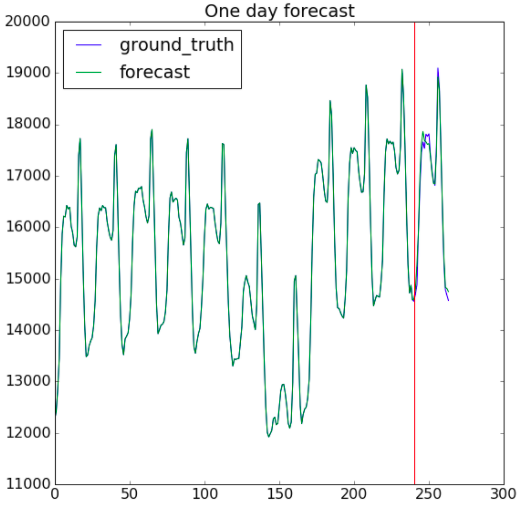
\includegraphics[width=\textwidth]{oneday.png}
    \end{subfigure}
    \begin{subfigure}[b]{0.3\textwidth}
        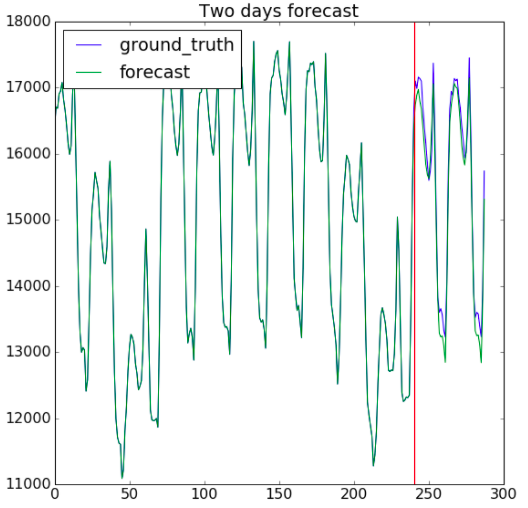
\includegraphics[width=\textwidth]{twodays.png}
    \end{subfigure}
    \begin{subfigure}[b]{0.3\textwidth}
        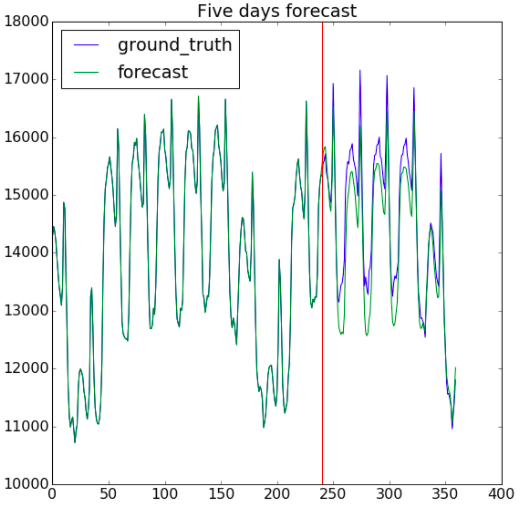
\includegraphics[width=\textwidth]{fivedays.png}
    \end{subfigure}
    \begin{subfigure}[b]{0.3\textwidth}
        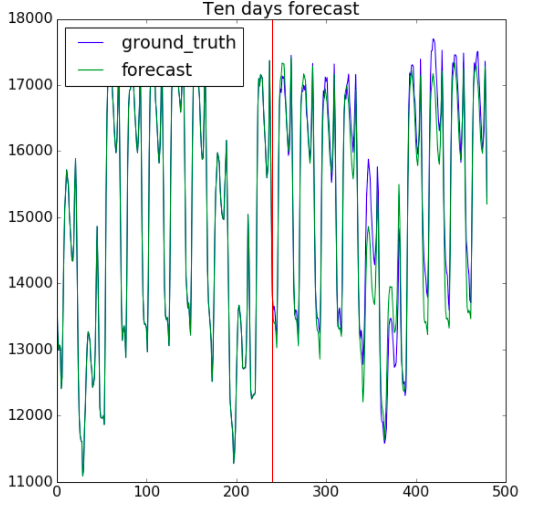
\includegraphics[width=\textwidth]{tendays.png}
    \end{subfigure}
    \begin{subfigure}[b]{0.3\textwidth}
        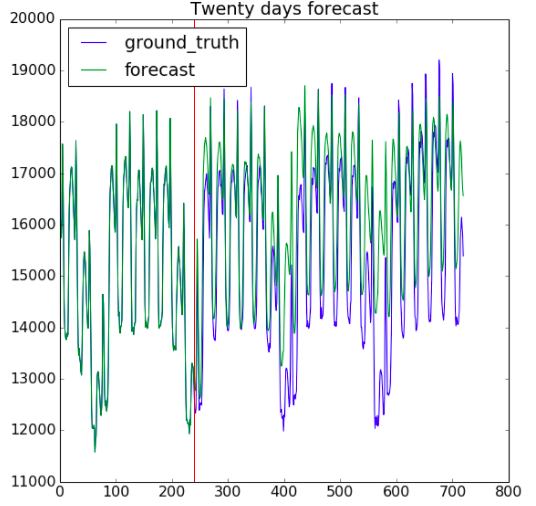
\includegraphics[width=\textwidth]{twentydays.png}
    \end{subfigure}
    \begin{subfigure}[b]{0.3\textwidth}
        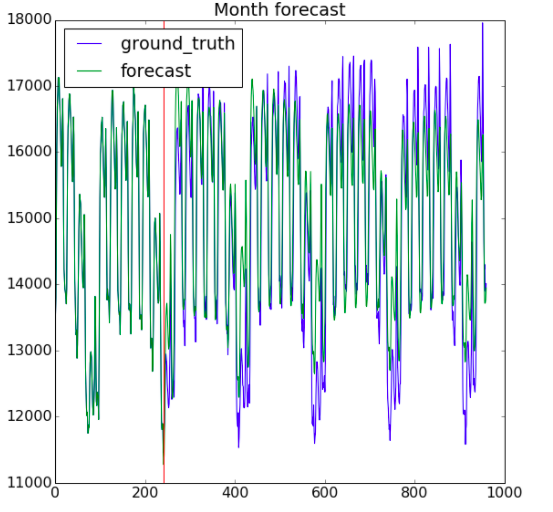
\includegraphics[width=\textwidth]{month.png}
    \end{subfigure}
    \caption{Прогнозирование базового алгоритма на 1, 2, 5, 10, 20, 30 дней}
    \label{fig:forecast}
\end{figure}

Результаты вычислительного эксперимента для предложенного модифицированного алгоритма cnlPLS представлены на рис.~\ref{fig:animals}. На графиках изображены сглаженные зависимости ошибки MSE от числа компонент в алгоритме для разных функций. Из графиков видно, что для функций $(a)-(e)$ ошибка при увеличении числа компонент падает, затем колеблется, слабо меняясь. Ошибка алгоритма с функцией $(f)$ увеличивается при увеличении числа компонент. Это означает, что преобразование, выполненное в пространстве целевой переменной с помощью функции $(f)$, плохо описывает зависимость. Меньшую ошибку имеют функции, растущие медленнее, а именно $(d)$ и $(e)$. 

\begin{figure}
    \centering
    \begin{subfigure}[b]{0.4\textwidth}
        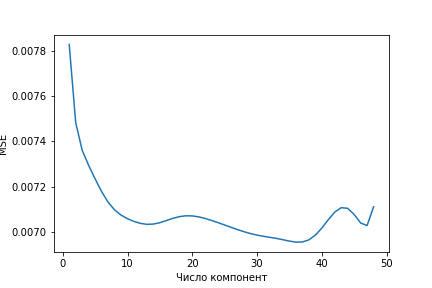
\includegraphics[width=\textwidth]{exp_abs_x.png}
        \caption{$g(x) = \sign(x) e^a(\exp(b|x|) - 1)$}
        \label{fig:exp_abs_x}
    \end{subfigure}
    ~ %add desired spacing between images, e. g. ~, \quad, \qquad, \hfill etc. 
      %(or a blank line to force the subfigure onto a new line)
    \begin{subfigure}[b]{0.4\textwidth}
        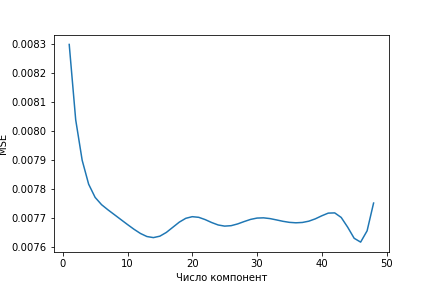
\includegraphics[width=\textwidth]{exp_log_x.png}
        \caption{$g(x) = \sign(x)e^a(\exp(b\ln(1+ \,|x|) - 1)$}
        \label{fig:exp_log_x}
    \end{subfigure}
    ~ %add desired spacing between images, e. g. ~, \quad, \qquad, \hfill etc. 
    %(or a blank line to force the subfigure onto a new line)
    \begin{subfigure}[b]{0.4\textwidth}
        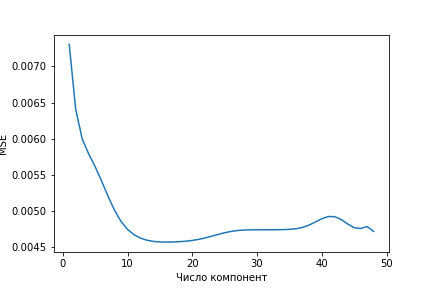
\includegraphics[width=\textwidth]{exp_x_1_2.png}
        \caption{$g(x) = \sign(x)e^a(\exp(b|x|^{1/2}) - 1)$}
        \label{fig:exp_x_1_2}
    \end{subfigure}
    \begin{subfigure}[b]{0.4\textwidth}
        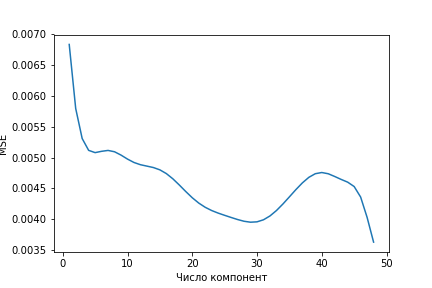
\includegraphics[width=\textwidth]{exp_x_1_3.png}
        \caption{$g(x) = \sign(x)e^a(\exp(b|x|^{1/3}) - 1)$ }
        \label{fig:exp_x_1_3}
    \end{subfigure}
    ~ %add desired spacing between images, e. g. ~, \quad, \qquad, \hfill etc. 
      %(or a blank line to force the subfigure onto a new line)
    \begin{subfigure}[b]{0.4\textwidth}
        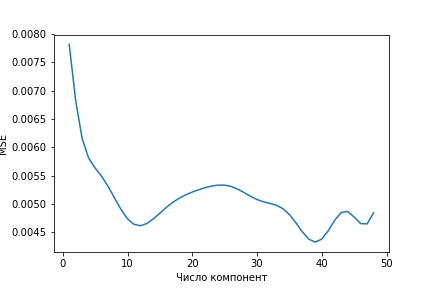
\includegraphics[width=\textwidth]{exp_x_1_4.png}
        \caption{$g(x) = \sign(x)e^a(\exp(b|x|^{1/4}) - 1)$}
        \label{fig:exp_x_1_4}
    \end{subfigure}
    ~ %add desired spacing between images, e. g. ~, \quad, \qquad, \hfill etc. 
    %(or a blank line to force the subfigure onto a new line)
    \begin{subfigure}[b]{0.4\textwidth}
        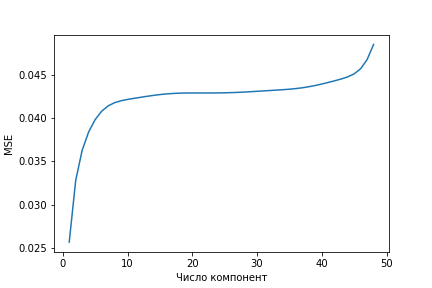
\includegraphics[width=\textwidth]{exp_x_2.png}
        \caption{$g(x) = \sign(x)e^a(\exp(b|x|^{2}) - 1)$}
        \label{fig:exp_x_2}
    \end{subfigure}
    \caption{Зависимость ошибки от числа компонент в алгоритме cnlPLS для разных функций}\label{fig:animals}
\end{figure}

В табл.~\ref{results} продемонстрировано увеличение точности прогнозивания при использовании криволинейного преобразования в пространстве зависимой переменной, но увеличение точности в пределах погрешности алгоритма (0.0005-0.0010). Функции с быстрым ростом не позволяют описать зависимость.
\begin{table}[]
\centering
\begin{tabular}{|l|l|l|l|l|}
\hline
\textbf{Алгоритм}                                                                                  & \textbf{N=3}     & \textbf{N=5}     & \textbf{N=10}    & \textbf{N=20}    \\ \hline
PLS                                                                                                & 0,00404          & 0,00337          & \textbf{0,00151} & 0,00135          \\ \hline
\begin{tabular}[c]{@{}l@{}}cnlPLS\\ $g(x) = \sign(x)\exp(a)(\exp(b|x|) - 1)$\end{tabular}          & 0.00529          & 0.00514          & 0.00536          & 0.00506          \\ \hline
\begin{tabular}[c]{@{}l@{}}cnlPLS\\ $g(x) = \sign(x)\exp(a)(\exp(b\ln(1+ \,|x|) - 1)$\end{tabular} & 0.00362          & 0.00386          & 0.00326          & 0.00317          \\ \hline
\begin{tabular}[c]{@{}l@{}}cnlPLS\\ $g(x) = \sign(x)\exp(a)(\exp(b|x|^{1/2}) - 1)$\end{tabular}    & 0.00272          & 0.00236          & 0.00287          & \textbf{0.00128} \\ \hline
\begin{tabular}[c]{@{}l@{}}cnlPLS\\ $g(x) = \sign(x)\exp(a)(\exp(b|x|^{1/3}) - 1)$\end{tabular}    & \textbf{0.00241} & \textbf{0.00233} & 0.00221          & 0.00173          \\ \hline
\begin{tabular}[c]{@{}l@{}}cnlPLS\\ $g(x) = \sign(x)\exp(a)(\exp(b|x|^{1/4}) - 1)$\end{tabular}    & 0.00796          & 0.00768          & 0.00737          & 0.00803          \\ \hline
\begin{tabular}[c]{@{}l@{}}cnlPLS\\ $g(x) = \sign(x)\exp(a)(\exp(b|x|^{2}) - 1)$\end{tabular}      & 0.00816          & 0.00798          & 0.00796          & 0.00775          \\ \hline
\end{tabular}
\caption{Значения ошибки MSE для разных чисел компонент и разных функций}
\label{results}
\end{table}

%%%%%%%%%%%%%%%%%%%%%%%%%%%%%%%%%%%%%%%%%%%%%%%%%%%%%%%%%%%%%%%%%%%%%%%%%%%%%%
\section{Заключение}
В данной работе предложен новый подход к обнаружению зависимостей в пространстве зависимой переменной задачи прогнозирования временных рядов. Сравнивались результаты прогнозирования временных рядов, полученных с помощью метода частных наименьших квадратов и предложенной модификации. Проведен вычислительный эксперимент на реальных данных потребления электроэнергии в Варшаве. Построенная прогностическая модель показала высокое качество предсказания электрической нагрузки. 
%%%%%%%%%%%%%%%%%%%%%%%%%%%%%%%%%%%%%%%%%%%%%%%%%%%%%%%%%%%%%%%%%%%%%%%%%%%%%%
%\section*{СПИСОК ЛИТЕРАТУРЫ}

%\bibliographystyle{gost71sv}
%\bibliography{MachLearn}
\newpage
\nocite{*}

\bibliographystyle{unsrt}
\bibliography{papers_pls.bib}
% \begin{thebibliography}{00}

% \bibitem{uspenskiy15amctm}
%     Uspenskiy\;V., Vorontsov\;K., Tselykh\;V., Bunakov\;V.
%     Information Function of the Heart:
%     Discrete and Fuzzy Encoding of the ECG-Signal for Multidisease Diagnostic System.
%     In~\emph{Advanced Mathematical and Computational Tools in Metrology and Testing X, Series on Advances in Mathematics for Applied Sciences}. 2015. World Scientific. Singapore. Vol.\,86. Pp. 377--384.
% \end{thebibliography}





\end{document} 